%%
%% Copyright 2026 Elsevier Ltd
%%
%% This file is part of the 'Elsarticle Bundle'.
%% ---------------------------------------------
%%
%% It may be distributed under the conditions of the LaTeX Project Public
%% License, either version 1.2 of this license or (at your option) any
%% later version.  The latest version of this license is in
%%    http://www.latex-project.org/lppl.txt
%% and version 1.2 or later is part of all distributions of LaTeX
%% version 1999/12/01 or later.
%%
%% The list of all files belonging to the 'Elsarticle Bundle' is
%% given in the file `manifest.txt'.
%%

%% Template article for Elsevier's document class `elsarticle'
%% with numbered style bibliographic references
%% SP 2008/03/01

\documentclass[preprint,12pt, a4paper]{elsarticle}

%% Use the option review to obtain double line spacing
%% \documentclass[authoryear,preprint,review,12pt]{elsarticle}

%% For including figures, graphicx.sty has been loaded in
%% elsarticle.cls. If you prefer to use the old commands
%% please give \usepackage{epsfig}

%% The amssymb package provides various useful mathematical symbols
\usepackage{amsmath}
\usepackage{amssymb}
\usepackage{amsfonts}

%% Tables
\usepackage{booktabs}
\usepackage{tabularx}
\usepackage{array}
\usepackage{multirow}

%% Lists, links, listings
\usepackage{enumitem}
\usepackage{hyperref}
\usepackage{xcolor}
\usepackage{listings}

\setlength{\parindent}{0pt}
%% The amsthm package provides extended theorem environments
%% \usepackage{amsthm}

%% The lineno packages adds line numbers. Start line numbering with
%% \begin{linenumbers}, end it with \end{linenumbers}. Or switch it on
%% for the whole article with \linenumbers.
%\usepackage{lineno}

%% ---- Listings style (transferred from the IEEE source) ---------------------
\definecolor{backgroundColour}{HTML}{F8F8F8}
\definecolor{keywordclr}{HTML}{AA00FF}
\definecolor{commentclr}{HTML}{649696}
\definecolor{stringsclr}{HTML}{11A579}
\lstdefinestyle{PythonStyle}{
    language=Python,
    backgroundcolor=\color{backgroundColour},
    keywordstyle=\color{keywordclr},
    stringstyle=\color{stringsclr},
    commentstyle=\color{commentclr},
    upquote=true,
    basicstyle=\ttfamily\linespread{0.9}\footnotesize,
    breakatwhitespace=false,
    breaklines=true,
    captionpos=b,
    keepspaces=true,
    numbers=left,
    numbersep=5pt,
    numberstyle=\color{commentclr}\ttfamily\tiny,
    showspaces=false,
    showstringspaces=false,
    showtabs=false,
    tabsize=2,
    xleftmargin=2.25em,
    frame=single,
    framexleftmargin=1.25em,
    morekeywords={assert,with,as,None}
}
\lstset{style=PythonStyle}

\journal{SoftwareX}

\begin{document}

\begin{frontmatter}

%% Title, authors and addresses

%% use the tnoteref command within \title for footnotes;
%% use the tnotetext command for theassociated footnote;
%% use the fnref command within \author or \address for footnotes;
%% use the fntext command for theassociated footnote;
%% use the corref command within \author for corresponding author footnotes;
%% use the cortext command for theassociated footnote;
%% use the ead command for the email address,
%% and the form \ead[url] for the home page:

\title{HiveWatch: Framework-Agnostic Observability for Federated and Distributed Machine Learning}

%% use optional labels to link authors explicitly to addresses:

\author[anl,umass]{Abhijit Chunduru}
\ead{schunduru@anl.gov}

\author[anl]{Zilinghan Li}
\ead{zilinghan.li@anl.gov}

\author[anl,uchicago]{Ravi Madduri\corref{cor1}}
\ead{madduri@anl.gov}

\cortext[cor1]{Corresponding author}

\address[anl]{Argonne National Laboratory, Lemont, IL, USA}
\address[umass]{University of Massachusetts Amherst, Amherst, MA, USA}
\address[uchicago]{The University of Chicago, Chicago, IL, USA}

\begin{abstract}
%% Text of abstract
We present HiveWatch, an open-source, framework-agnostic observability toolkit for federated and distributed machine learning. HiveWatch provides a five-call runtime API and an FL-native event schema covering round starts, per-client updates, round summaries, communication metadata, system resource utilization, client geography, and failure events. A pluggable emitter interface simultaneously forwards the same event stream to local replayable JSONL artifacts and a map dashboard (SSEEmitter), Weights \& Biases (WandbEmitter), and MLflow (MLflowEmitter). We demonstrate integration into three FL frameworks with different communication stacks — APPFL, Flower, and NVIDIA FLARE — using the same API in each case. A microbenchmark shows that internal bookkeeping adds 5--37\,$\mu$s per call, with the disk-persisting emitter adding $\sim$2.8\,ms per call, negligible relative to typical FL round durations.
\end{abstract}

\begin{keyword}
%% keywords here, in the form: keyword \sep keyword
Federated Learning \sep Distributed Machine Learning \sep Observability \sep Experiment Tracking \sep MLflow \sep Weights and Biases \sep Map Visualization \sep Software

%% PACS codes here, in the form: \PACS code \sep code

%% MSC codes here, in the form: \MSC code \sep code
%% or \MSC[2008] code \sep code (2000 is the default)

\end{keyword}

\end{frontmatter}

%\linenumbers

\section*{Required Metadata}
\label{}

\section*{Current code version}
\label{}

Ancillary data table required for subversion of the codebase. Kindly replace examples in right column with the correct information about your current code, and leave the left column as it is.

\begin{table}[!h]
\begin{tabular}{|l|p{4.5cm}|p{7.5cm}|}
\hline
\textbf{Nr.} & \textbf{Code metadata description} & \textbf{Please fill in this column} \\
\hline
C1 & Current code version & v0.2.1 \\
\hline
C2 & Permanent GitHub link to code/repository used for this code version & \url{https://github.com/APPFL/hivewatch/releases/tag/v0.2.1} \\
\hline
C3 & Legal Code License   & MIT License \\
\hline
C4 & Code versioning system used & git \\
\hline
C5 & Software code languages, tools, and services used & Python\,$\geq$\,3.8; optional extras: \texttt{wandb}\,$\geq$\,0.16 (Weights \& Biases backend), \texttt{mlflow}\,$\geq$\,2.0 (MLflow backend), \texttt{requests}\,$\geq$\,2.25 (client geolocation helpers); no mandatory third-party dependencies for the core package \\
\hline
C6 & Compilation requirements, operating environments \& dependencies & \texttt{pip install hivewatch} from source or PyPI; Linux, macOS, Windows; no compilation step required; full dependency specification in \texttt{pyproject.toml} \\
\hline
C7 & If available Link to developer documentation/manual & \url{https://appfl.github.io/hivewatch/}; runnable examples for APPFL, Flower, and NVIDIA FLARE in \texttt{examples/} at the repository root \\
\hline
C8 & Support email for questions & \{schunduru, zilinghan.li, madduri\}@anl.gov \\
\hline
\end{tabular}
\caption{Code metadata (mandatory)}
\label{tab:codemeta}
\end{table}

\textbf{Main text}\\

\section{Motivation and significance}
\label{sec:motivation}
Federated learning (FL) is a distributed machine learning paradigm that enables multiple clients to collaboratively train models without sharing raw data~\cite{mcmahan2017communication}, making it particularly valuable in privacy-sensitive domains such as healthcare~\cite{rieke2020future}, edge computing~\cite{lim2020federated}, and multi-institutional research~\cite{kairouz2021advances}. As FL deployments grow in scale, they introduce a distinct \emph{observability} challenge that existing tooling does not address. A single training run can involve many geographically distributed clients with heterogeneous data distributions, compute capabilities, communication costs, and failure modes~\cite{li2020federated}. Without a unified monitoring layer, practitioners must manually reconcile disparate logs, re-implement per-client metric schemas for each new project, and hard-code a choice of monitoring backend up front.

General-purpose experiment tracking tools — Weights \& Biases~\cite{wandb}, MLflow~\cite{mlflow}, and TensorBoard~\cite{tensorboard} — are effective for centralized training but have no native notion of a federated round, a client population, per-client staleness, or client geography. Adapting them to FL typically means hand-rolling a per-project naming scheme for per-client metrics and recomputing derived quantities such as gradient divergence and communication volume in every codebase. Modern FL frameworks — APPFL~\cite{ryu2022appfl,li2025advances}, Flower~\cite{beutel2020flower}, NVIDIA FLARE~\cite{roth2022nvidia}, and FedML~\cite{he2020fedml} — each ship their own logging facilities, but these are tightly coupled to the framework's runtime. Switching frameworks means re-learning a different logging surface and rebuilding custom dashboards. Research on heterogeneity and straggler management~\cite{lai2021oort,li2024fedcompass,xie2019asynchronous,nguyen2022federated} defines \emph{what} to measure in FL but does not provide \emph{how to measure it} in a portable way.

HiveWatch addresses this gap. It provides a framework-agnostic runtime API and an FL-native event schema — covering round starts, per-client updates, round summaries, failures, and checkpoints — that sits between any FL framework and any combination of monitoring backends. The same instrumentation code can simultaneously stream experiment data to local replayable artifacts, Weights \& Biases, and MLflow, with derived metrics such as gradient divergence, byte totals, and per-round wall time computed once inside HiveWatch and forwarded to every configured backend. The goal is to separate the \emph{what} of observability (the FL-specific schema) from the \emph{where} (the choice of backend), so that practitioners can instrument once and monitor anywhere.
s

\section{Software description}
\label{sec:software}

\subsection{Software Architecture}

As shown in Fig.~\ref{fig:hivewatch}, HiveWatch is designed as a server-side instrumentation layer that sits between an existing federated learning framework and one or more monitoring backends. The FL framework remains fully responsible for client selection, model distribution, local training, and aggregation. HiveWatch is inserted at the server's control flow, where it records events and forwards them to emitter backends without modifying the underlying communication protocol or aggregation algorithm. This separation allows HiveWatch to support APPFL, Flower, NVIDIA FLARE, and custom training loops with no changes to HiveWatch itself.

\begin{figure*}[t]
    \centering
    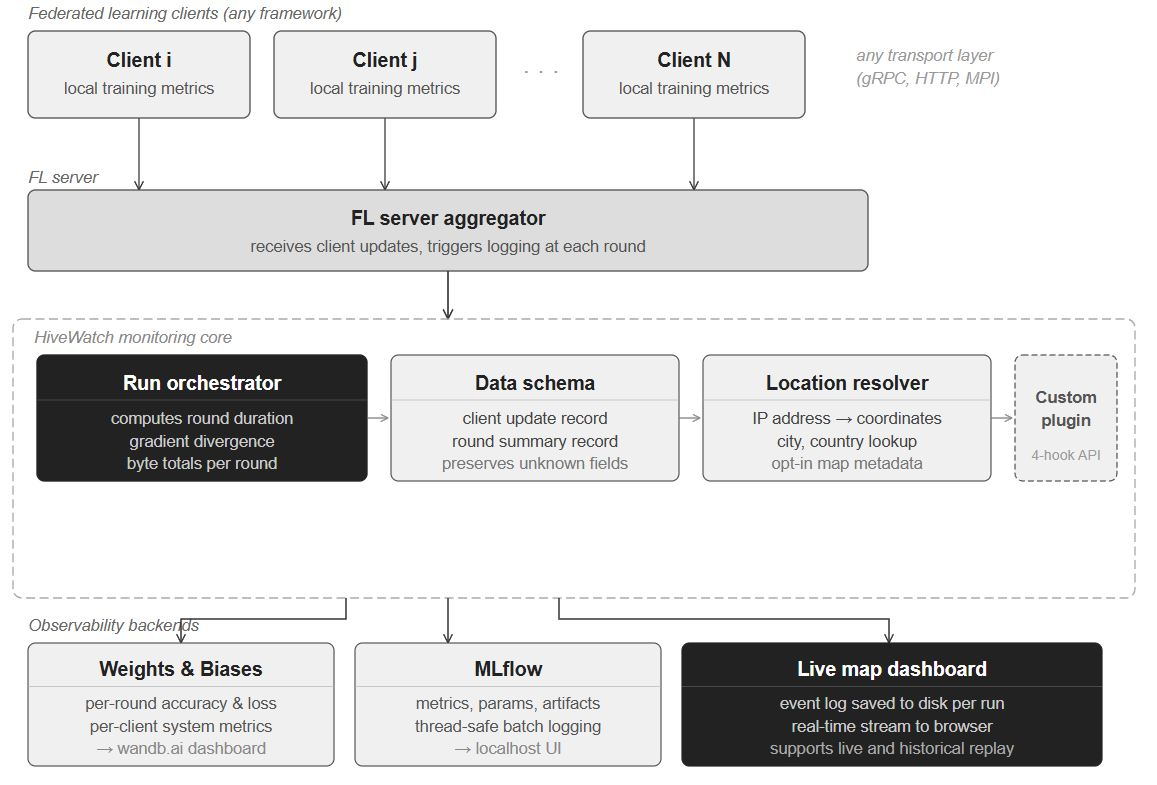
\includegraphics[width=0.9\linewidth]{images/arch.JPG}
    \caption{HiveWatch monitoring framework. The FL server calls the HiveWatch runtime API; events are fanned out to local JSONL artifacts, a map dashboard, MLflow, and Weights \& Biases simultaneously.}
    \label{fig:hivewatch}
\end{figure*}

\subsection{Software Functionalities}

\textbf{Runtime API.}
HiveWatch exposes five primary calls, listed in Table~\ref{tab:api}. During each training round the server marks the round start, records each client update as it arrives, and logs the final round-level summary after aggregation.

\begin{table}[t]
\caption{HiveWatch runtime API.}
\label{tab:api}
\centering
\begin{tabular}{ll}
\toprule
\textbf{Call} & \textbf{When to invoke} \\
\midrule
\texttt{hivewatch.init(\ldots)} & Once at server startup \\
\texttt{round\_start(round)} & Start of each global round \\
\texttt{log\_client\_update(id, **kw)} & Each client result received \\
\texttt{log\_round(round, \ldots)} & After aggregation \\
\texttt{finish()} & Server shutdown \\
\bottomrule
\end{tabular}
\end{table}

\textbf{Event Schema.}
Client updates may include local accuracy, local loss, number of samples, gradient norm and sparsity, bytes sent and received, training wall time, CPU, RAM and GPU utilization, geographic metadata (\texttt{lat}/\texttt{lng}/\texttt{country}), and asynchronous staleness (\texttt{base\_round}). Unknown framework-specific fields are preserved verbatim. Round summaries capture global accuracy and loss, per-round wall time, the number of clients selected and completed (from which emitters derive a participation rate), straggler and failure counts, total communication volume, gradient divergence (standard deviation of per-client gradient norms), and aggregation time. Derived quantities — gradient divergence, byte totals, round wall time — are computed once inside HiveWatch and forwarded to every configured backend.

\textbf{Emitter Backends.}
HiveWatch decouples metric collection from metric storage through a pluggable emitter interface. Arbitrary numbers of emitters may be attached simultaneously:

\begin{itemize}[noitemsep]
    \item \textbf{SSEEmitter:} Appends every event to a replayable JSONL event log and rewrites a map-ready \texttt{.map.json} snapshot on every call. Artifacts survive process crashes and enable full post-hoc replay without re-running training.
    \item \textbf{WandbEmitter:} Logs per-client and per-round metrics to Weights \& Biases, using \texttt{wandb.define\_metric()} to align all series on the round axis.
    \item \textbf{MLflowEmitter:} Records metrics, parameters, tags, and model checkpoint artifacts to a local or remote MLflow tracking server. Per-client keys use dot notation to comply with MLflow naming conventions.
\end{itemize}

Custom emitters may be added by implementing four methods: \texttt{on\_init}, \texttt{on\_round}, \texttt{on\_client\_update}, and \texttt{finish}.

\textbf{Map Dashboard.}
The SSEEmitter artifact can be served by the bundled \texttt{hivewatch map run} CLI, which provides a local browser-based dashboard visualising client locations, training status, round progress, straggler markers, and per-client sidebar metadata. Both live runs (streamed via server-sent events) and completed runs (replayed from saved artifacts) are supported.

\subsection{Implementation Notes}

HiveWatch is a pure-Python package (Python~$\geq$~3.8) released under the MIT license. The core package has no mandatory third-party dependencies beyond the standard library. Weights~\&~Biases and MLflow support, and the optional client geolocation helper used by the map dashboard, are installed as extras via \texttt{pip install hivewatch[wandb]}, \texttt{[mlflow]}, \texttt{[geo]}, or \texttt{[all]}. Internal bookkeeping uses a single \texttt{threading.Lock} so that \texttt{log\_client\_update()} is safe to call from concurrent server threads. The package ships the map dashboard HTML file as a package data asset; no build step or web bundler is required.

\section{Illustrative examples}
\label{sec:illustrative}

\subsection{Installation and Quickstart}

HiveWatch is installed from PyPI in a single command:

\begin{lstlisting}[style=PythonStyle,language=bash,caption={Installation.}]
pip install hivewatch            # core only, no third-party deps
pip install hivewatch[all]       # with W&B, MLflow, and geolocation
\end{lstlisting}

The following listing shows a minimal integration of HiveWatch into any FL server loop, requiring no knowledge of the underlying framework:

\begin{lstlisting}[style=PythonStyle,caption={Minimal HiveWatch integration.}]
import hivewatch
from hivewatch.emitters import SSEEmitter, WandbEmitter

hivewatch.init(
    algorithm="FedAvg",
    emitters=[
        SSEEmitter(runs_dir="runs", port=7070),
        WandbEmitter(project="my-fl-project"),
    ],
)

for round_num in range(num_rounds):
    hivewatch.round_start(round_num)

    for client_id, result in client_results.items():
        hivewatch.log_client_update(
            client_id,
            round=round_num,
            local_accuracy=result["acc"],
            local_loss=result["loss"],
            num_samples=result["n"],
            bytes_sent=result["bytes"],
            train_time_sec=result["t"],
        )

    hivewatch.log_round(
        round_num,
        global_accuracy=agg_acc,
        global_loss=agg_loss,
    )

hivewatch.finish()
\end{lstlisting}

\subsection{Framework Integration}

We demonstrate framework-agnosticism by integrating the identical five-call API into three FL frameworks with different communication stacks. Full runnable examples ship with the HiveWatch source distribution.

\textit{APPFL (gRPC).} The APPFL example subclasses \texttt{ServerAgent} and intercepts each client update in \texttt{global\_update()}, calling \texttt{round\_start()} on each round transition and \texttt{log\_client\_update()} after aggregation returns. Every HiveWatch runtime call is made on the server.

\textit{Flower.} The Flower example subclasses \texttt{FedAvg}, forwarding per-client metrics carried in Flower's \texttt{FitRes} objects to \texttt{log\_client\_update()} from \texttt{aggregate\_fit()}, and logging the round summary from \texttt{aggregate\_evaluate()} once the global metrics are available. Failed clients reported by Flower are recorded through \texttt{log\_dropout()}.

\textit{NVIDIA FLARE.} The NVIDIA FLARE example subclasses \texttt{FedAvg} to inject HiveWatch calls into \texttt{send\_model()}, \texttt{\_aggregate\_one\_result()}, and \texttt{\_get\_aggregated\_result()}, and swaps the wrapped controller into the recipe's deployment map.

The bridging layer is confined to a single server-side file per framework --- approximately 75 lines for APPFL and Flower, and 115 for NVIDIA FLARE, whose controller must additionally be reconstructed and swapped into the recipe's deployment map --- and none of the three required any modification to HiveWatch itself. Clients otherwise remain framework-native: the Flower example touches no HiveWatch code on the client at all, populating only Flower's own \texttt{fit()} metrics dictionary, which the strategy then forwards. The single optional client-side addition is a call to HiveWatch's \texttt{get\_location()} helper when geographic metadata is wanted for the map dashboard; the APPFL and NVIDIA FLARE examples use it to tag each update with the client's coordinates.

\subsection{Instrumentation Overhead}

Because HiveWatch runs on the server's critical path, its overhead must be small relative to typical round durations. We measure per-call overhead over 50 rounds with 20 clients per round (1{,}050 calls total), comparing no-emitter (bookkeeping only) and SSEEmitter (synchronous JSONL append plus full \texttt{.map.json} rewrite per call) configurations. The workload is synthetic --- no model, dataset, or FL framework is involved --- so the reported times reflect instrumentation cost alone. The measurement script ships with the repository as \texttt{benchmarks/instrumentation\_overhead.py}, so the table can be regenerated on any machine. Results are shown in Table~\ref{tab:overhead}.

\begin{table}[t]
\caption{Per-call instrumentation overhead ($\mu$s), 50 rounds $\times$ 20 clients.}
\label{tab:overhead}
\centering
\begin{tabular}{lrrr}
\toprule
\textbf{Call (configuration)} & \textbf{Mean} & \textbf{Median} & \textbf{p95} \\
\midrule
\texttt{log\_client\_update} (no emitter) & 5.0 & 4.7 & 5.9 \\
\texttt{log\_round} (no emitter)           & 37.2 & 34.3 & 48.9 \\
\texttt{log\_client\_update} (SSEEmitter)  & 2822.5 & 2759.0 & 4763.8 \\
\texttt{log\_round} (SSEEmitter)           & 3005.4 & 2995.7 & 4723.7 \\
\bottomrule
\end{tabular}
\end{table}

Internal bookkeeping (schema normalization, derived-metric computation, round-state tracking) costs 5--37\,$\mu$s per call regardless of which emitters are attached. The SSEEmitter raises per-call overhead to $\sim$2.8\,ms, which is entirely attributable to the synchronous file flush after each JSONL append and the full rewrite of the map metadata snapshot — a deliberate consistency tradeoff so that crashed runs leave a complete, replayable artifact on disk. Summed over a 20-client round, the SSEEmitter adds $\sim$59\,ms of server overhead, which is negligible relative to real FL round durations (seconds to minutes). The WandbEmitter and MLflowEmitter offload persistence to external services and do not incur per-call file I/O. The SSEEmitter produced a 1.09\,MB JSONL history file and a 439\,KB map metadata snapshot for this 50-round, 20-client workload — sufficient to fully reconstruct client geography, status transitions, and round summaries via the map dashboard without re-running training.

\section{Impact}
\label{sec:impact}
HiveWatch enables three classes of practitioner activity that are not well served by existing tooling.

\textbf{Portable instrumentation across FL frameworks.} Researchers who work with multiple FL frameworks — or who plan to migrate from one to another — currently must re-implement per-project monitoring code for each framework. HiveWatch provides a single instrumentation target that works across APPFL, Flower, NVIDIA FLARE, and custom training loops, reducing the instrumentation burden to five call sites regardless of which framework is used.

\textbf{Simultaneous multi-backend monitoring.} Teams frequently need to publish experiment results to more than one destination: local artifacts for immediate debugging, a hosted dashboard for cross-run comparison, and a self-hosted tracking server for compliance or reproducibility. HiveWatch's emitter model supports this with no duplication of instrumentation logic, and the SSEEmitter's replayable JSONL artifacts ensure that a run can be inspected offline after the fact without re-running training.

\textbf{FL-native diagnostics.} HiveWatch's schema captures straggler counts, gradient divergence (as a proxy for data heterogeneity), per-client staleness in asynchronous FL, communication volume breakdowns, client dropout and failure events, and geographic client metadata — none of which are available without per-project custom code when using general-purpose tracking tools such as Weights \& Biases or MLflow directly. These signals are the inputs to algorithmic heterogeneity-mitigation methods~\cite{lai2021oort,li2024fedcompass,xie2019asynchronous}, and having them logged consistently enables practitioners to characterize and diagnose heterogeneity before choosing which mitigation to apply.

The primary audience is FL practitioners and researchers who need reproducible, inspectable experiment records across diverse FL deployments — including multi-institutional biomedical FL~\cite{rieke2020future}, edge FL~\cite{lim2020federated}, and academic FL benchmarking. HiveWatch is released under the MIT license, is developed in the open at \url{https://github.com/APPFL/hivewatch} with documentation at \url{https://appfl.github.io/hivewatch/}, and is installable from PyPI with a single \texttt{pip install hivewatch} command.

\section{Conclusions}
\label{sec:conclusion}
We presented HiveWatch, a lightweight, framework-agnostic observability layer for federated and distributed ML. By defining an FL-native event schema and decoupling metric collection from metric storage through a pluggable emitter interface, HiveWatch lets the same five-call instrumentation simultaneously stream to local replayable JSONL artifacts, Weights \& Biases, and MLflow. We demonstrated this by integrating HiveWatch into APPFL, Flower, and NVIDIA FLARE using the same server-side API in each case, and showed through a microbenchmark that per-call instrumentation overhead is 5--37\,$\mu$s for internal bookkeeping alone and $\sim$2.8\,ms with the disk-persisting SSEEmitter — a small fraction of a typical FL round duration.

Current limitations include a single-machine map server intended for local debugging rather than production multi-user dashboards, and the requirement that applications map framework-specific result fields to HiveWatch's schema at the bridging layer. Future work includes additional emitters (Prometheus, TensorBoard), lightweight anomaly flagging for gradient drift or communication degradation, and cross-run comparison views in the map dashboard.

%% ---- Declarations ----------------------------------------------------------
% ---- CRediT Author Contribution Statement ----------------------------------
\section*{CRediT Author Contribution Statement}
\textbf{Abhijit Chunduru:} Conceptualization, Software, Validation, Writing -- original draft, Writing -- review and editing.
\textbf{Zilinghan Li:} Conceptualization, Software, Validation, Writing -- original draft, Writing -- review and editing.
\textbf{Ravi Madduri:} Supervision, Funding acquisition, Writing -- review and editing.

% ---- Data Availability ------------------------------------------------------
\section*{Data Availability}
HiveWatch does not process or distribute datasets. The software source code, runnable examples, and documentation are publicly available at \url{https://github.com/APPFL/hivewatch} under the MIT license. No experimental datasets were used in producing the results in this paper; the instrumentation overhead figures were obtained by running the bundled hivewatch package in a synthetic microbenchmark with no external data.

% ---- Declaration of Competing Interests -------------------------------------
\section*{Declaration of Competing Interests}
The authors declare that they have no known competing financial interests or personal relationships that could have appeared to influence the work reported in this paper.

% ---- Declaration of Generative AI ------------------------------------------
\section*{Declaration of Generative AI and AI-Assisted Technologies}
During the preparation of this work, the authors used Anthropic Claude to support manuscript drafting and structural review. The authors reviewed, verified, and edited all outputs and take full responsibility for the content of the published article.

\section*{Acknowledgements}
\label{}
This material is based upon work supported by the U.S.\ Department of Energy, Office of Science, under contract number DE-AC02-06CH11357. We also gratefully acknowledge Amazon Web Services for providing cloud computing credits that supported the experimental work for this manuscript.

%% The Appendices part is started with the command \appendix;
%% appendix sections are then done as normal sections
%% \appendix

%% \section{}
%% \label{}

%% References:
%% If you have bibdatabase file and want bibtex to generate the
%% bibitems, please use

\bibliographystyle{elsarticle-num}
\bibliography{references}

\section*{Current executable software version}
\label{}

\begin{table}[!h]
\begin{tabular}{|l|p{4.5cm}|p{7.5cm}|}
\hline
\textbf{Nr.} & \textbf{(Executable) software metadata description} & \textbf{Please fill in this column} \\
\hline
S1 & Current software version & v0.2.1 \\
\hline
S2 & Permanent link to executables of this version & \url{https://github.com/APPFL/hivewatch/releases/tag/v0.2.1}; installable via \texttt{pip install hivewatch} \textcolor{red}{how to add dependency here} \\
\hline
S3 & Legal Software License & MIT License \\
\hline
S4 & Computing platforms/Operating Systems & Linux, macOS, Windows (Python\,$\geq$\,3.8) \\
\hline
S5 & Installation requirements \& dependencies & \texttt{pip install hivewatch}; optional extras: \texttt{wandb\,$\geq$\,0.16}, \texttt{mlflow\,$\geq$\,2.0}, \texttt{requests}\,$\geq$\,2.25  \\
\hline
S6 & If available, link to user manual & \url{https://hivewatch.readthedocs.io};\\
\hline
S7 & Support email for questions & \{schunduru, zilinghan.li, madduri\}@anl.gov \\
\hline
\end{tabular}
\caption{Software metadata}
\label{tab:softwaremeta}
\end{table}

\end{document}
\endinput
%%
%% End of file `SoftwareX_article_template.tex'.
